\documentclass{article}
\usepackage[latin1]{inputenc}
\usepackage{tikz}
\usetikzlibrary{shapes,arrows}
\usepackage{caption}
\newcommand*{\h}{\hspace{5pt}}% for indentation
\newcommand*{\hh}{\h\h}% double indentation
\begin{document}
\begin{center}
  \sffamily
  \footnotesize
  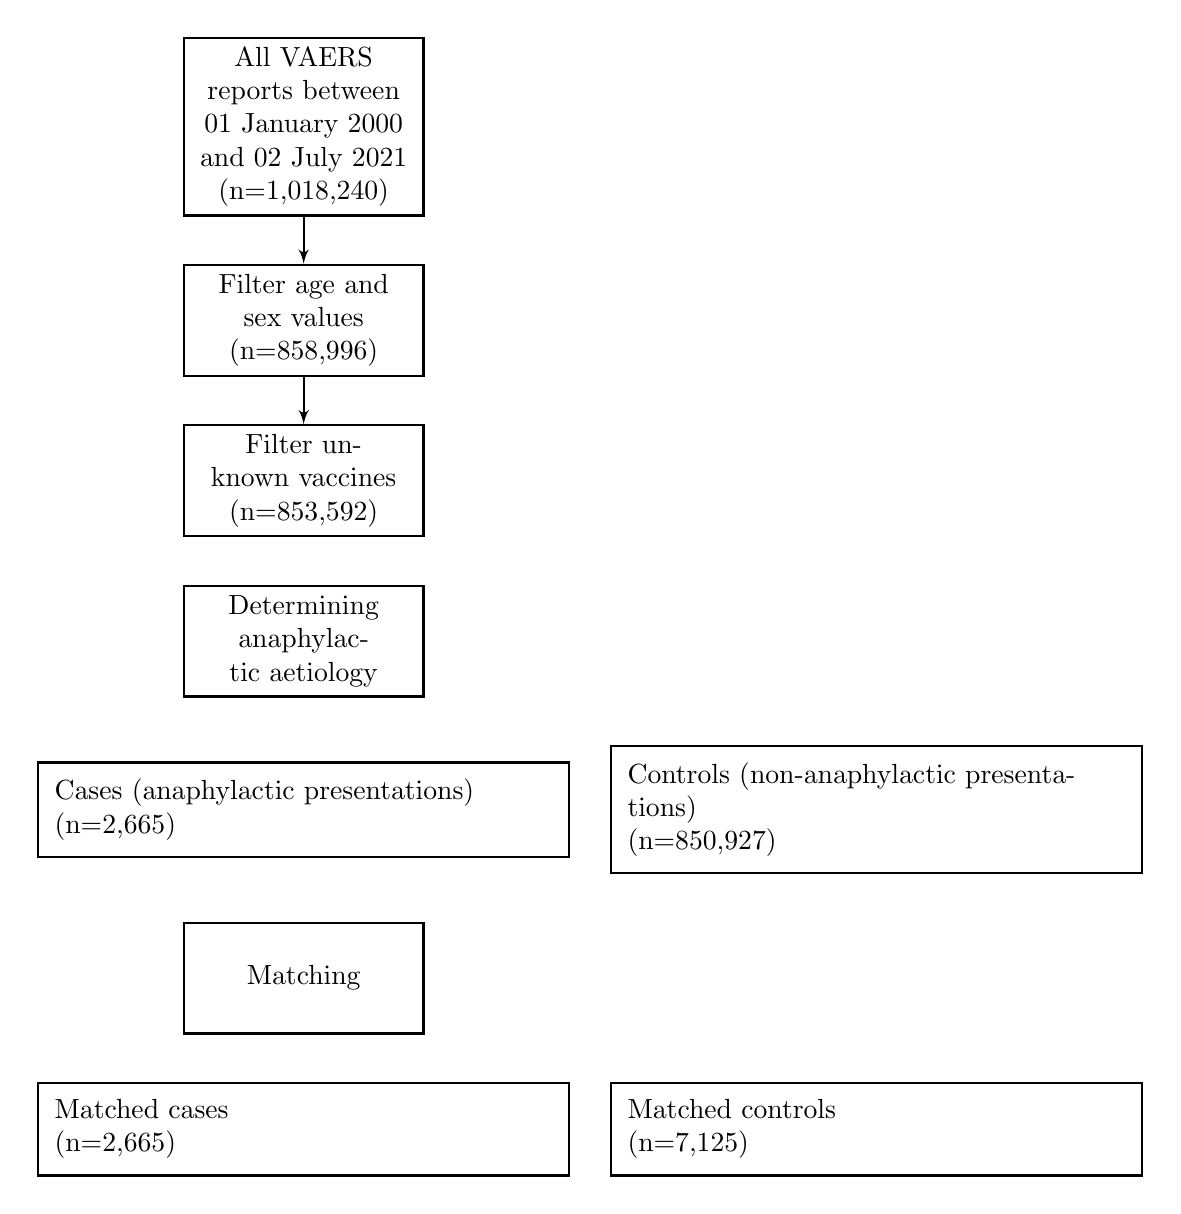
\begin{tikzpicture}[auto,
    %decision/.style={diamond, draw=black, thick, fill=white,
    %text width=8em, text badly centered,
    %inner sep=1pt, font=\sffamily\small},
    block_center/.style ={rectangle, draw=black, thick, fill=white,
      text width=8em, text centered,
      minimum height=4em},
    block_left/.style ={rectangle, draw=black, thick, fill=white,
      text width=16em, text ragged, minimum height=4em, inner sep=6pt},
    block_noborder/.style ={rectangle, draw=none, thick, fill=none,
      text width=18em, text centered, minimum height=1em},
    block_assign/.style ={rectangle, draw=black, thick, fill=white,
      text width=18em, text ragged, minimum height=3em, inner sep=6pt},
    block_lost/.style ={rectangle, draw=black, thick, fill=white,
      text width=16em, text ragged, minimum height=3em, inner sep=6pt},
      line/.style ={draw, thick, -latex', shorten >=0pt}]
    % outlining the flowchart using the PGF/TikZ matrix funtion
    \matrix [column sep=5mm,row sep=6mm] {
      % row 1
      \node [block_center] (loaded_vaers) {All VAERS reports between 01 January 2000 and 02 July 2021 (n=1,018,240)}; \\
      \node [block_center] (filter_age_sex) {Filter age and sex values (n=858,996)}; \\
      \node [block_center] (filter_unknown_vax) {Filter unknown vaccines (n=853,592)}; \\
      \node [block_center] (anaphylaxis) {Determining anaphylactic aetiology}; \\
      \node [block_assign] (cases) {Cases (anaphylactic presentations)\\(n=2,665)};
      & \node [block_assign] (controls) {Controls (non-anaphylactic presentations)\\(n=850,927)}; \\
      \node [block_center] (matching) {Matching}; \\
      \node [block_assign] (matched_cases) {Matched cases\\(n=2,665)};
      & \node [block_assign] (matched_controls) {Matched controls\\(n=7,125)}; \\
    };% end matrix
    % connecting nodes with paths
    \begin{scope}[every path/.style=line]
      \path (loaded_vaers)   -- (filter_age_sex);
      \path (filter_age_sex)   -- (filter_unknown_vax);
    \end{scope}
  \end{tikzpicture}
\end{center}
\end{document}